\section{FreshQA Public Main And Sequence: Volatile Public Boundary}

The official FreshQA public runs are the most important boundary evidence in the paper. They test the same controller on frozen public changing-answer data derived from weekly releases, once on a changed-question-heavy main slice and once on a sequence slice with repeated corrections and forgetting probes. Across all four models, the headline result is consistent: retrieval dominates, and suppressing delayed utility is more reliable than softly calibrating it. The accompanying manual audit found 24 clean cases, 76 suspect cases, and no direct leakage-risk cases, so the benchmark is useful and auditable but not fully trust-cleared.

\subsection{Main slice}

\begin{table}[h]
\centering
\small
\begin{tabular}{llrrrrr}
\toprule
Model & Policy & Quality & 95\% CI & Retrieve & Adapt & Stale \\
\midrule
FLAN-T5 Base & Retrieval only & 1.000 & [1.000, 1.000] & 796.0 & 0.0 & 0.000 \\
FLAN-T5 Base & Retrieve gate & 0.132 & [0.132, 0.132] & 89.0 & 0.0 & 0.005 \\
FLAN-T5 Base & Full router & 0.616 & [0.544, 0.687] & 448.6 & 69.8 & 0.002 \\
FLAN-T5 Base & Calibrated router & 0.694 & [0.634, 0.754] & 528.4 & 18.0 & 0.001 \\
FLAN-T5 Base & Router without delayed utility & 0.985 & [0.985, 0.985] & 740.0 & 4.0 & 0.000 \\
FLAN-T5 Small & Retrieval only & 1.000 & [1.000, 1.000] & 796.0 & 0.0 & 0.000 \\
FLAN-T5 Small & Retrieve gate & 0.134 & [0.134, 0.134] & 89.0 & 0.0 & 0.003 \\
FLAN-T5 Small & Full router & 0.612 & [0.539, 0.684] & 448.6 & 69.8 & 0.001 \\
FLAN-T5 Small & Calibrated router & 0.794 & [0.725, 0.863] & 612.4 & 29.4 & 0.000 \\
FLAN-T5 Small & Router without delayed utility & 0.984 & [0.984, 0.984] & 739.0 & 4.0 & 0.000 \\
\bottomrule
\end{tabular}

\caption{Official FreshQA public main results on the primary FLAN matrix. Retrieval is perfect; calibration partially repairs the full router, but the no-\(V_{\text{future}}\) ablation remains much closer to the retrieval ceiling.}
\label{tab:public-freshqa-main}
\end{table}

On the main slice, \texttt{always\_retrieve} is 1.000 on both FLAN backbones and remains 1.000 on Qwen2.5-1.5B and SmolLM2 as well. The full router falls to 0.616 on FLAN-T5-Base and 0.612 on FLAN-T5-Small. Calibration helps relative to the full router, reaching 0.694 and 0.794, but the no-\(V_{\text{future}}\) ablation (\texttt{router\_no\_v\_future}) is still far stronger at 0.985 and 0.984. The paired sign tests are decisive: retrieval beats the full router, the calibrated router, and the no-\(V_{\text{future}}\) ablation on both FLAN models, while the no-\(V_{\text{future}}\) ablation strongly beats both router variants.

\begin{figure}[h]
\centering
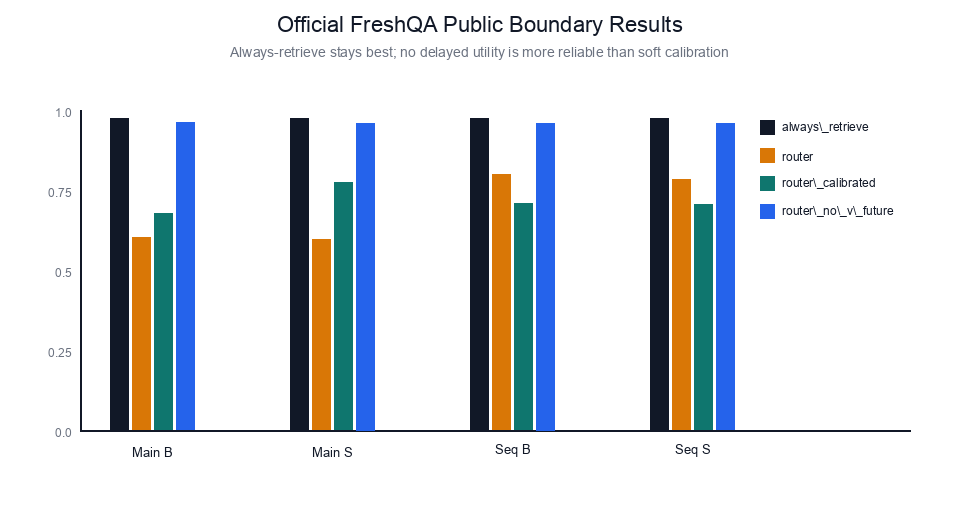
\includegraphics[width=0.95\linewidth]{../shared/generated/word_assets/fig_public_main_calibration_curve.png}
\caption{Official public-boundary comparison on the primary FLAN matrix. Retrieval is perfect on both FreshQA public slices, while the no-\(V_{\text{future}}\) ablation stays much closer to that ceiling than the full or calibrated router.}
\label{fig:public-best-mode}
\end{figure}

\clearpage
\subsection{Sequence slice}

\begin{table}[h]
\centering
\small
\begin{tabular}{llrrrrr}
\toprule
Model & Policy & Quality & 95\% CI & Retrieve & Adapt & Stale \\
\midrule
FLAN-T5 Base & Retrieval only & 1.000 & [1.000, 1.000] & 796.0 & 0.0 & 0.000 \\
FLAN-T5 Base & Retrieve gate & 0.132 & [0.132, 0.132] & 89.0 & 0.0 & 0.005 \\
FLAN-T5 Base & Full router & 0.819 & [0.708, 0.930] & 630.0 & 84.6 & 0.000 \\
FLAN-T5 Base & Calibrated router & 0.725 & [0.647, 0.804] & 540.6 & 26.4 & 0.000 \\
FLAN-T5 Base & Router without delayed utility & 0.984 & [0.984, 0.984] & 739.0 & 5.0 & 0.000 \\
FLAN-T5 Small & Retrieval only & 1.000 & [1.000, 1.000] & 796.0 & 0.0 & 0.000 \\
FLAN-T5 Small & Retrieve gate & 0.134 & [0.134, 0.134] & 89.0 & 0.0 & 0.003 \\
FLAN-T5 Small & Full router & 0.802 & [0.687, 0.916] & 614.0 & 82.0 & 0.000 \\
FLAN-T5 Small & Calibrated router & 0.724 & [0.643, 0.804] & 539.2 & 26.6 & 0.000 \\
FLAN-T5 Small & Router without delayed utility & 0.982 & [0.982, 0.982] & 738.0 & 5.0 & 0.000 \\
\bottomrule
\end{tabular}

\caption{Official FreshQA public sequence results on the primary FLAN matrix. On repeated correction chains, suppressing delayed utility is again much safer than the full router, and soft calibration is inconsistent.}
\label{tab:public-freshqa-sequence}
\end{table}

The sequence slice sharpens the same conclusion. Retrieval again stays at 1.000, while the full router reaches 0.819 on FLAN-T5-Base and 0.802 on FLAN-T5-Small. Here calibration is not heroic; it is worse than the full router on both primary FLAN models, falling to 0.725 and 0.724. The no-\(V_{\text{future}}\) ablation again stays much closer to retrieval at 0.984 and 0.982, and the corresponding sign tests show it significantly outperforming both router variants. The cross-family appendix extends the same qualitative pattern to Qwen2.5-1.5B and SmolLM2.

\begin{table}[h]
\centering
\small
\begin{tabular}{lr}
\toprule
Audit field & Count \\
\midrule
Always-retrieve correct / router wrong & 40 \\
Always-retrieve correct / calibrated-router wrong & 25 \\
Alias-heavy or multi-answer & 20 \\
Rollback / forgetting / answer-change probes & 15 \\
\midrule
Clean verdicts & 24 \\
Suspect verdicts & 76 \\
Leakage-risk verdicts & 0 \\
\bottomrule
\end{tabular}

\caption{Official FreshQA manual audit summary. The audit found no direct leakage-risk cases, but many cases remain suspect, so the public trust story is bounded rather than fully cleared.}
\label{tab:public-audit}
\end{table}

The manual audit matters for interpretation. Among 100 audited cases, 24 were labeled clean, 76 were labeled suspect, and none were labeled direct leakage risk. That is enough to reject a simple leakage explanation for the retrieval-dominant result, but not enough to treat the benchmark as fully cleared. The right conclusion is modest: public changing-answer evaluation is hard, retrieval is the safest policy in our current setup, and delayed utility should usually be suppressed rather than softly calibrated in this regime.
